\documentclass[a4paper]{tufte-handout}
\setcounter{secnumdepth}{1}
\geometry{paperwidth=186mm,paperheight=297mm,left=12.8mm,top=27.4mm,headsep=2\baselineskip,textwidth=107mm,marginparsep=8.2mm,marginparwidth=49.4mm,textheight=49\baselineskip,headheight=\baselineskip}

%% \usepackage{biolinum}
%% \usepackage{eulervm}     % AMS Euler math font.

%% Tufte uses titlesec. titlesec < 2.10.2 has a bug that prevents showing
%% section numbers. This fixes it. Taken from
%% https://tex.stackexchange.com/questions/96090/formatting-subsections-and-chapters-in-tufte-book/96125
\usepackage{etoolbox}
\makeatletter
\patchcmd{\ttlh@hang}{\parindent\z@}{\parindent\z@\leavevmode}{}{}
\patchcmd{\ttlh@hang}{\noindent}{}{}{}
\makeatother

\titleformat{\section}%
  {\normalfont\Large\itshape}% format applied to label+text
  {\llap{\parbox{1cm}{\hfill\itshape\Large\thesection}\hspace*{0.5cm}}}% label
  {2pt}% horizontal separation between label and title body
  {}% before the title body
  []% after the title body

%% \titleformat{\subsection}%
%%   {\normalfont\large\itshape}% format applied to label+text
%%   {\llap{\parbox{1cm}{\hfill\itshape\large\thesubsection\hspace*{0.2cm}}}}% label
%%   {2pt}% horizontal separation between label and title body
%%   {}% before the title body
%%   []% after the title body

%% ---- Packages ----
\usepackage{amssymb,amsmath,amsthm,latexsym}
\usepackage{mathpartir}
\usepackage{multirow}
\usepackage{url,hyperref}
\usepackage{stmaryrd}           % for semantic brackets
\usepackage{mathtools}          % for \dblcolon
\usepackage{accents}            % for \underaccent
\usepackage{tikz,tikz-cd}       % Hasse & commutative diagrams.
\usepackage{adjustbox}          % aligning tikz diagrams vertically w/ tables.p


%% ---- Commands ----
\newtheorem{theorem}{Theorem}
\newtheorem{definition}{Definition}

\newcommand{\todo}[1]{{\color{red}#1}}

\newcommand{\bnfeq}{\dblcolon=}
\newcommand{\defeq}{\overset{\ms{def}}{=}}

\newcommand{\ms}[1]{\ensuremath{\mathsf{#1}}}
\newcommand{\mb}[1]{\ensuremath{\mathbf{#1}}}
\newcommand{\mi}[1]{\ensuremath{\mathit{#1}}}
\newcommand{\mc}[1]{\ensuremath{\mathcal{#1}}}

\newcommand{\GG}{\Gamma}

\newcommand{\N}{\mathbb{N}}
\newcommand{\x}{\times}
\newcommand{\fn}{\lambda}
\newcommand{\binder}{.\,}
\newcommand{\bind}[1]{{#1}\binder}
\newcommand{\sub}[1]{\{{#1}\}}
\newcommand{\fix}{\ms{fix}}

%% TODO: get rid of \Disc, \Codisc.
\newcommand{\Disc}{{\color{red}\square}}
\newcommand{\Codisc}{{\color{red}\lozenge}}

\newcommand{\den}[1]{\llbracket{#1}\rrbracket}

%% Category & preorder theory
\newcommand{\id}{\ms{id}}
\newcommand{\op}{\ms{op}}
\newcommand{\iso}{\ms{core}}
\renewcommand{\path}{\ms{path}}

\newcommand{\isoto}{\simeq}
\newcommand{\pathto}{\sim}

%% tones: mono, anti, discrete, bivariant
\newcommand{\tm}{\id}                        % monotone / id
\newcommand{\ta}{{\color{ForestGreen}\op}}   % antitone / op
\newcommand{\ti}{{\color{NavyBlue}\iso}}     % invariant/ core
\newcommand{\tb}{{\color{Bittersweet}\path}} % bivariant/ path

\newcommand{\tc}{\cdot}         % tone composition

\newcommand{\h}[3]{#1 : {#2}^{#3}}
\newcommand{\hm}[2]{\h{#1}{#2}{\tm}}
\newcommand{\ha}[2]{\h{#1}{#2}{\ta}}
\newcommand{\hi}[2]{\h{#1}{#2}{\ti}}
\newcommand{\hb}[2]{\h{#1}{#2}{\tb}}

\newcommand{\mto}{\overset{\tm}{\to}}
\newcommand{\ato}{\overset{\ta}{\to}}
\newcommand{\ito}{\overset{\ti}{\to}}
\newcommand{\bto}{\overset{\tb}{\to}}


%% ---- Front matter ----
\title{Tones and Types}
%% alternate title: Tone theory
%% alternate title: Tonality inference
\author{Michael Arntzenius}
%% \email{daekharel@gmail.com}
\date{16 November 2017 -- ???}


\begin{document}
\maketitle

\section{A preamble on preorders}

A preorder is a relation $a \le b$ satisfying:
\begin{enumerate}
\item \textbf{Reflexivity:} $a \le a$.
\item \textbf{Transitivity:} If $a \le b$ and $b \le c$ then $a \le c$.
\end{enumerate}

\marginnote{To a category theorist, a preorder is a ``thin'' category: between
  any two objects there is at most one morphism. I suspect much of the ``tone
  theory'' in this document, ostensibly about maps between preorders, extends to
  functors between categories.}

A good example is ``lists under containment'', where $a \le b$ iff every element
of $a$ is also in $b$.

Preorders are partial orders, sans antisymmetry. Let $a \equiv b$ iff $a \le b$
and $b \le a$. Antisymmetry means $a \equiv b$ implies $a = b$. However, under
list containment, $[0,1] \equiv [1,0]$, but $[0,1] \ne [1,0]$.


\subsection{Tones (categorically)}

\todo{TODO: this note is useful, but should go somewhere else}

\newcommand{\elemset}[1]{\ensuremath{\mc{U}({#1})}}
\newcommand{\elemsetfn}[0]{\mc{U}}
\renewcommand{\elemset}[1]{\ensuremath{|{#1}|}}
\renewcommand{\elemsetfn}[0]{\elemset{-}}

Let $\elemsetfn{} : \mb{Preorder} \to \mb{Set}$ be the forgetful functor that
takes a preorder to its set of elements.

\begin{definition}
  A tone $s$ is a functor $-^s : \mb{Preorder} \to \mb{Preorder}$ such that
  $\elemset{-^s} = \elemsetfn$.
\end{definition}

\marginnote{A more ``categorical'' definition might require only a natural
  isomorphism $\iota : \elemset{-^s} \isoto \elemsetfn$. I'm not comfortable
  generalizing that far yet.}

In particular, for any preorder $A$ and monotone map $f$,
\begin{enumerate}
\item $|A^s| = |A|$, i.e. a tone functor transforms only the \emph{ordering},
  not the elements, of a preorder.
\item $|f^s| = |f|$, i.e. a tone functor does not change the behavior of
  functions.
\end{enumerate}


\section{Tones}

Tones are ways a function $f$ may respect a preordering. I will consider four
tones, \tm, \ta, \tb, and \ti{}:

\begin{center}
  \begin{tabular}{clc@{\hskip 0.25em}c@{\hskip 0.25em}c}
    \multicolumn{1}{c}{\textbf{Tone}}
    & \multicolumn{1}{c}{\textbf{Name}}
    %% & \multicolumn{1}{c}{\textbf{Respects}}
    & \multicolumn{3}{c}{\textbf{Property of $f$}}
    \\\hline
    \tm & \text{Monotone}
    %% & \text{ordering}
    & $x \le y$ &$\implies$& $f(x) \le f(y)$
    \\
    \ta & \text{Antitone}
    %% & \text{opposite ordering}
    & $x \ge y$ &$\implies$& $f(x) \le f(y)$
    \\
    \tb & \text{Bivariant}
    %% & \text{equivalence closure or ``paths''}
    & $x \le y \vee y \le x$ &$\implies$& $f(x) \le f(y)$
    \\
    \ti & \text{Invariant}
    %% & \text{induced equivalence or ``isomorphisms''}
    & $x \le y \wedge y \le x$ &$\implies$& $f(x) \le f(y)$
  \end{tabular}
  \vspace{0.5em}
\end{center}

\noindent Informally,
\begin{enumerate}
\item $\tm$ is monotone, or order-preserving.
\item $\ta$ is antitone, or order-inverting.
\item $\tb$ is bivariant: both monotone and antitone.
\item $\ti$ is invariant, preserving only equivalence.\marginnote{In posets,
  antisymmetry trivializes invariance, because $x \le y \wedge y \le x$ implies
  $x = y$, thus $f(x) = f(y)$.}
\end{enumerate}


\subsection{Tones transform orders}

Consider preorders $A, B$. Let $A^\op$ be $A$, ordered oppositely. Now, observe
that

\begin{center}
  $f : A \to B$ is antitone

  \emph{iff}

  $f : A^\op \to B$ is monotone
\end{center}

So ``antitone'' is a special case of ``monotone''! This observation generalizes:
every tone is really monotonicity with a transformation applied to the domain's
ordering. So \textbf{tones transform orders.}
%
I write $A^s$ for the preorder $A$ transformed by the tone $s$, defined by:

\begin{fullwidth}
  \vspace{1em}
  \begin{tabular}{clc@{\hskip 0.25em}c@{\hskip 0.25em}l}
    {\textbf{Tone}}
    & {\textbf{Meaning}}
    & \multicolumn{3}{c}{\textbf{Transformation on $A$}%
      \phantom{\small\quad\emph{``Defining \path{}''}}}
    \\\hline
    \tm & \text{same ordering}
    & $a \le b : A$ &$\iff$& $a \le b : A^\tm$
    \\
    \ta
    & \text{opposite ordering}
    & $a \ge b : A$ &$\iff$& $a \le b : A^\op$
    \\
    \tb{}
    & \text{equivalence closure}
    & $a \le b \vee b \le a : A$ &$\ \implies$& $a \le b : A^\path$
    \small\quad\emph{see ``Defining \path{}''}
    \\
    \ti
    & \text{induced equivalence}
    & $a \le b \wedge b \le a : A$ &$\iff$& $a \le b : A^\iso$
  \end{tabular}
  \vspace{1em}
\end{fullwidth}

With this, we can state the theorem generalizing our observation:
\begin{theorem}[Tones transform orders]\label{thm:tones-transform-orders}
  %% For any function $f : A \to B$ between preorders $A$, $B$:
  ~
  \begin{center}
    $f : A \to B$ has tone $s$

    \emph{iff}

    $f : A^s \to B$ is monotone
  \end{center}
\end{theorem}
%% \begin{proof} Exercise for the reader. \end{proof}

From this point on, when I write $f : A \to B$, I mean implicitly that $f$ is
monotone; and therefore $f : A^s \to B$ means that $f$ has tone $s$.
%
Also, there is one more property of tones we will need:

\begin{theorem}[Functoriality of tones]\label{thm:tone-functoriality}
  If $f : A \to B$ then $f : A^s \to B^s$.
  %% \[\text{If}~ f : A \to B ~\text{then}~ f : A^s \to B^s\text{.}\]
\end{theorem}
%% \begin{proof} Exercise for the reader. \end{proof}

%% Together, these theorems define a more general notion of tone: a tone $s$ is a
%% transformation $-^s$ on the ordering component of a preorder (i.e. $A^s$ must
%% have the same elements as $A$) satisfying Theorem \ref{thm:tone-functoriality},
%% whose interpretation as a property of functions is given by Theorem
%% \ref{thm:tones-transform-orders}.

\subsection{Defining \ms{path}} \label{sec:defining-path}

$A^\path$ is the smallest preorder satisfying
\[ a \le b \vee b \le a : A \implies a \le b : A^\path \]

Unfortunately $A^\path$ is not so easy to define directly (without
language like ``the smallest preorder satisfying'')
%
because the reverse implication, from $a \le b : A^\path$ to $a \le b \vee b \le
a : A$, does not always hold. A good counterexample is the \ms{fencepost}
ordering on the naturals, where $a \le a+1$ for even $a$, and $a \ge a+1$ for
odd $a$:

\todo{TODO: Diagram}.

Note that $a \le b \vee b \le a : \ms{fencepost} \iff |a-b| \le 1$, which isn't
transitive! Instead, $\ms{fencepost}^\path$ is the \emph{transitive closure} of
$|a-b| \le 1$, which makes everything equivalent:
\[ 0 \equiv 1 \equiv 2 \equiv 3 \equiv 4 \equiv ... \]

However, a direct definition of $A^\path$ is possible using \emph{paths}:
``zig-zagging'' lists $a_0, a_1, ..., a_n$ such that $a_i \le a_{i+1} \vee a_i
\ge a_{i+1} : A$. Then $a \le b : A^\path$ iff there is a path starting at $a$
and ending at $b$.


\subsection{Tone operators}

\begin{figure*}[t]
  \vspace{-3em}
  \begin{mathpar}
    %% "baseline=(current bounding box.center)" incantation taken from
    %% https://tex.stackexchange.com/questions/220531/how-to-align-tikzpicture-and-text-in-a-table/220543#220543
    %% \begin{tikzpicture}[baseline=(current bounding box.center)]
    %%   \node (top)  at ( 0, 1) {$\tb$};
    %%   \node (bot)  at ( 0,-1) {$\ti$};
    %%   \node (-1)   at (-1, 0) {$\tm$};
    %%   \node (1)    at ( 1, 0) {$\ta$};
    %%   \draw (top) -- (-1) -- (bot) -- (1) -- (top);
    %% \end{tikzpicture}
    %    
    %% \begin{array}{c|rrrrr}
    %%   s \wedge t & \tm & \tb & \ta & \ti\\\hline
    %%   \tm & \tm & \tm & \ti & \ti\\
    %%   \tb & \tm & \tb & \ta & \ti\\
    %%   \ta & \ti & \ta & \ta & \ti\\
    %%   \ti & \ti & \ti & \ti & \ti
    %% \end{array}
    %
    \begin{array}{cc|rrrrr}
      \multicolumn{2}{c|}{\multirow{2}{*}{$s \wedge t$}}
      & \multicolumn{4}{c}{t}\\
      && \tm & \tb & \ta & \ti\\\hline
      \multirow{4}{*}{$s$}
      & \tm & \tm & \tm & \ti & \ti\\
      & \tb & \tm & \tb & \ta & \ti\\
      & \ta & \ti & \ta & \ta & \ti\\
      & \ti & \ti & \ti & \ti & \ti
    \end{array}

    \begin{array}{cc|rrrr}
      \multicolumn{2}{c|}{\multirow{2}{*}{$s \tc t$}}
      & \multicolumn{4}{c}{t}\\
      && \tm & \ta & \ti & \tb\\\hline
      \multirow{4}{*}{$s$}
      & \tm & \tm & \ta & \ti & \tb\\
      & \ta & \ta & \tm & \ti & \tb\\
      & \ti & \ti & \ti & \ti & \ti\\
      & \tb & \tb & \tb & \tb & \tb
    \end{array}
  \end{mathpar}
  \caption{Tone meet and composition}
  \label{fig:tone-ops}
\end{figure*}

Figure \ref{fig:tone-ops} defines two operators on tones:
\begin{enumerate}
\item 
  Meet $s \wedge t$ is greatest lower bound in the tone lattice (Figure
  \ref{fig:tone-lattice}). This gives the general tone of the pairing $\langle
  f, g\rangle : A^{s \wedge t} \to B \times C$ of two functions $f : A^s \to B$
  and $g : A^{t} \to C$.
  %
  \begin{marginfigure}
    \normalsize
    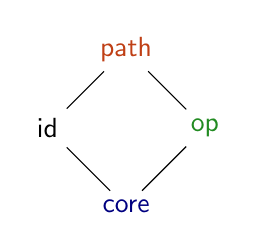
\begin{tikzpicture}[baseline=(current bounding box.center)]
      \node (top)  at ( 0, 1) {$\tb$};
      \node (bot)  at ( 0,-1) {$\ti$};
      \node (-1)   at (-1, 0) {$\tm$};
      \node (1)    at ( 1, 0) {$\ta$};
      \draw (top) -- (-1) -- (bot) -- (1) -- (top);
    \end{tikzpicture}
    \vspace{0.2cm}
    \caption{The tone lattice}
    \label{fig:tone-lattice}
  \end{marginfigure}

  %% \[\begin{array}{c|rrrrr}
  %% s \wedge t & \tm & \tb & \ta & \ti\\\hline
  %% \tm & \tm & \tm & \ti & \ti\\
  %% \tb & \tm & \tb & \ta & \ti\\
  %% \ta & \ti & \ta & \ta & \ti\\
  %% \ti & \ti & \ti & \ti & \ti
  %% \end{array}\]

  \todo{TODO: isn't this just intersection of the relations? if $R(a,b)$ and
    $S(a,b)$ are preorders, is $R(a,b) \wedge S(a,b)$ reflexive and transitive?
    Yes (even though $R(a,b) \vee S(a,b)$ isn't always)! So then $x \le y : A^{s
      \wedge t} \iff x \le y : A^s \wedge x \le y : A^t$?}

\item Composition $s \tc t$ gives the tone of a composed function $g \circ f :
  A^{s\tc t} \to C$ when $f : A^s \to B$ and $g : B^t \to C$. Equivalently,
  $A^{s\tc t} = (A^s)^t$ for any preorder $A$.

  %% \[\begin{array}{cc|rrrr}
  %% \multicolumn{2}{c|}{\multirow{2}{*}{$s \tc t$}}
  %% & \multicolumn{4}{c}{t}\\
  %% && \tm & \ta & \ti & \tb\\\hline
  %% \multirow{4}{*}{$s$}
  %% & \tm & \tm & \ta & \ti & \tb\\
  %% & \ta & \ta & \tm & \ti & \tb\\
  %% & \ti & \ti & \ti & \ti & \ti\\
  %% & \tb & \tb & \tb & \tb & \tb
  %% \end{array}\]

  \todo{TODO: Likewise, this is just observing that tones compose to tones,
    right? But does this semantic operation match up with our syntactic
    definition of $s \tc t$?}
\end{enumerate}



Together, $\wedge$ and $\tc$ form a semiring, satisfying the following panoply
of laws:
\begin{fullwidth}
  \begin{mathpar}
    \begin{array}{lr@{\hskip 0.5em}c@{\hskip 0.5em}l}
      \multicolumn{4}{c}{\textbf{Properties of } \wedge}
      \vspace{0.1em}\\
      \textbf{Associativity} & (s \wedge t) \wedge u &=& s \wedge (t \wedge u)\\
      \textbf{Commutativity} & s \wedge t &=& t \wedge s\\
      \textbf{Idempotence} & s \wedge s &=& s\\
      \tb~\textbf{is identity} & \tb \wedge s &=& s\\
      \ti~\textbf{absorbs} & \ti \wedge s &=& \ti\\
    \end{array}

    \begin{array}{lr@{\hskip 0.5em}c@{\hskip 0.5em}l}
      \multicolumn{4}{c}{\textbf{Properties of } \tc}
      \vspace{0.1em}\\
      \textbf{Associativity} & (s \tc t) \tc u &=& s \tc (t \tc u)\\
      \textbf{Identity} & \multicolumn{3}{c}{\tm \tc s = s = s \tc \tm}\\
      \tb~ \textbf{left-absorbs} & \tb \tc s &=& \tb\\
      \ti~ \textbf{left-absorbs} & \ti \tc s &=& \ti\\
      \ta~ \textbf{self-inverts} & \ta \tc \ta &=& \tm\\
    \end{array}

    \begin{array}{lr@{\hskip 0.5em}c@{\hskip 0.5em}l}
      \textbf{Left-distribution} & s \tc (t \wedge u) &=& (s \tc t) \wedge (s \tc u)\\
      \textbf{Right-distribution} & (s \wedge t) \tc u &=& (s \tc u) \wedge (t \tc u)
    \end{array}
  \end{mathpar}
\end{fullwidth}

\todo{TODO: Reference ``I Got Plenty o' Nuttin'{}'' ---
  another use of variable annotations drawn from a semiring, and with similar
  (the same?) behavior of those annotations in the inference rules.}

\subsection{Relation to Monotonicity Types}

\href{https://infoscience.epfl.ch/record/231867/files/monotonicity-types.pdf}{\emph{Monotonicity
    Types}} by Clancy, Miller, and Meiklejohn has similar tables for their
composition $\circ$ and ``contraction'' $+$ operators! However, instead of
bivariance they have constancy, a stricter condition.
%
Constancy corresponds to respecting the \emph{indiscrete ordering} (which sets
$a \le b$ for all $a,b$).\marginnote{Indiscreteness and its dual, discreteness,
  are also tones --- that is, functorial transformations on the ordering
  component of a preorder --- but they complicate things, so I omit them.

  Also worth noting is that discreteness and $\ti$ coincide when restricted to
  posets; many intuitions transfer from one to the other.}
%
Interestingly, because constancy is so much stricter than bivariance, their
composition operator is commutative.

They write $\uparrow$ for $\tm$, $\downarrow$ for $\ta$, $?$ for $\ti$, and
$\sim$ for constancy. They also add $=$ for the ``tone'' that \emph{only the
  identity function} has. This doesn't fit my framework; it cannot be phrased as
a transformation on orderings. However, it seems related to subtyping.



\section{A tonal sequent calculus}


  \begin{mathpar}
    (A_1^{t_1}, ..., A_n^{t_n})^u = (A_1^{t_1 \tc u}, ..., A_n^{t_n \tc u})\\

    \infer[$T$-Right]{\GG \vdash A}{\GG^t \vdash T_t A}

    \infer[$T$-Left]{\GG{},A^{t\tc u} \vdash C}{\GG{}, (T_t A)^u \vdash C}

    \infer[Weakening]{\GG{}, A^t \vdash C \quad u \le t}{\GG{}, A^u \vdash C}

    \infer[Contraction]{\GG{},A^t, A^u \vdash C}{\GG{}, A^{t \wedge u} \vdash C}

    \infer[Cut]{\GG \vdash A \quad \Delta,A^t \vdash C}{\GG^t,\Delta \vdash C}
  \end{mathpar}

Jason Reed sent me these rules for a tonal sequent calculus. $T_s$ is the
connective to internalizing $-^s$. I aim to adapt this into a
natural-deduction-style system with proof terms, i.e.\! a simply typed
$\lambda$-calculus.

\todo{TODO: Revisit this. Think about what $T$-Left means, and Kevin Clancy's
  phrasing of the eliminator for his type as requiring tones compose to
  something $\le \tm$.}


\FloatBarrier
\section{A bidirectional $\lambda$-calculus with tone inference}

\newcommand{\isfn}[4]{{#2}^{#1}\sqsubset {#3} \Rightarrow {#4}}
\newcommand{\subtype}[3]{{#2}^{#1}\sqsubset {#3}}
\newcommand{\converts}[3]{{#2}^{#1} \prec {#3}}

\newcommand{\infers}[3]{{#1}\vdash {#2} ~\mb{infers}~ {#3}}
\newcommand{\checks}[3]{{#1}\vdash {#2} ~\mb{checks}~ {#3}}

\renewcommand{\infers}[3]{{#2} \Rightarrow {#1} \vdash {#3}}
\renewcommand{\checks}[3]{{#2} \Leftarrow {#1} \vdash {#3}}

\begin{fullwidth}
  \begin{mathpar}
    \begin{array}{cccl}
      \text{tones} & s,t,u & \bnfeq & \tm ~|~ \ta ~|~ \tb ~|~ \ti
      \vspace{0.5em}\\
      \text{types} & A,B,C
      &\bnfeq& \ms{base} ~|~ A \to B ~|~ A \x B ~|~ \Box A ~|~ \op\;A
      \vspace{0.5em}\\
      \text{checking terms} & M
      &\bnfeq& N ~|~ \fn\bind{x} M ~|~ (M, M)
      ~|~ \mb{let}~x = N~\mb{in}~ M
      \vspace{0.5em}\\
      \text{inferring terms} & N
      &\bnfeq& M : A ~|~ x ~|~ N\;M ~|~ \pi_i\;N
      \vspace{0.5em}\\
      \text{contexts}
      & \GG &\bnfeq& \cdot ~|~ \GG{}, \h{x}{A}{s}
      \vspace{0.5em}\\
      \text{judgments}
      & J &\bnfeq&
      \checks{\GG}{M}{A}
      \\&&|& \infers{\GG}{N}{A}
      \\&&|& \subtype{s}{A}{B} ~|~ \converts{s}{A}{B}
    \end{array}
  \end{mathpar}
\end{fullwidth}

\todo{TODO: explain my various abuses of notation, e.g. $\GG^t$ and $\GG_1
  \wedge \GG_2$}

\todo{TODO: patterns and pattern inference}

\begin{fullwidth}
  \begin{mathpar}
    \infer{\quad}{\infers{\h{x}{A}{\tm}}{x}{A}}

    \infer{\checks{\GG}{M}{A}}{\infers{\GG}{M : A}{A}}

    \infer{\infers{\GG}{N}{A} \quad \subtype{t}{A}{B}}
          {\checks{\GG^t}{N}{B}}

    %% type-driven subtyping for checking
    \infer{\checks{\GG}{M}{A}}
          {\checks{\GG^\ti}{M}{\Box A}}

    \infer{\checks{\GG}{M}{A}}
          {\checks{\GG^\ta}{M}{\op\; A}}

    %% let-binding
    \infer{\infers{\GG_1}{N}{A} \quad \checks{\GG_2,\, \h{x}{A}{s}}{M}{C}}
          {\checks{\GG_1^s \wedge \GG_2}{\mb{let}~x = N~\mb{in}~M}{C}}

    %% introductions
    \infer{\checks{\GG{},\, \h{x}{A}{t}}{M}{B}
           \quad \subtype{s}{A}{A}
           \quad \tm \le s \tc t}
          {\checks{\GG}{\fn\bind{x} M}{A \to B}}

    \infer{\checks{\GG_1}{M_1}{A_1} \quad \checks{\GG_2}{M_2}{A_2}}
          {\checks{\GG_1 \wedge \GG_2}{(M_1,M_2)}{A_1 \x A_2}}

    %% eliminations
    \infer{\infers{\GG_1}{N}{A}
           \quad \converts{u}{A}{B \to C}
           \quad \checks{\GG_2}{M}{B}}
          {\infers{\GG_1^u \wedge \GG_2}{N\; M}{C}}

    \infer{\infers{\GG}{N}{A} \quad \converts{s}{A}{B_1 \x B_2}}
          {\infers{\GG^s}{\pi_i\;N}{B_i}}
  \end{mathpar}
\end{fullwidth}



\end{document}
